\subsection{Liskovs Substitution Principle}
    Liskov Substitution Principle states the following: " If for each object A of type S
    there is an object B of type T such that for all programs P defined in terms of T,
    the behavior of P is unchanged when A is substituted for B then S is a subtype of T"  
    \cite{Hotop2015}. This principle is taken into careful consideration for design 
    because it gives us the flexibility to replace the implementation in the dependent 
    class without modifying the other objects coupled to it. 
    \par
        Following Figure \ref{fig:navigationManagerClassDiagram} the attributes declared
        in this class are i.e. IDirectionApi, IGPSservice (the I prefix in a notation is for
        an interface) which are just abstractions instead of the concrete classes.
        Designing it in this way it would be possible to replace GoogleDirectionAPI service
        with any other realization and the Navigation manager would not see the difference.
        The only criteria is the concrete implementation should implement the interface
        which is exposed. An Example can be seen in the Listing \ref{code:liskovExample}

        \newpage
        \begin{lstlisting}[
            caption={Example of Liskovs susbstitution},
            label={code:liskovExample},
            language=java
            ]
            public class GoogleDirectionApiService implements IDirectionApi{}

            public interface IDirectionApi {
                void getDirections(final String mode, 
                    final String origin, final String destination, 
                    final String key, 
                    final Map<String,String> queries);
                void setOnProcessFinish(IAsyncTaskListenerOnFinish listner);
            }

            public class NavigationManger  implements INavigationManager {
             IDirectionApi googleDirectionApiService
            }
             
        \end{lstlisting} 

    \begin{figure}[htbp!]
        \centering 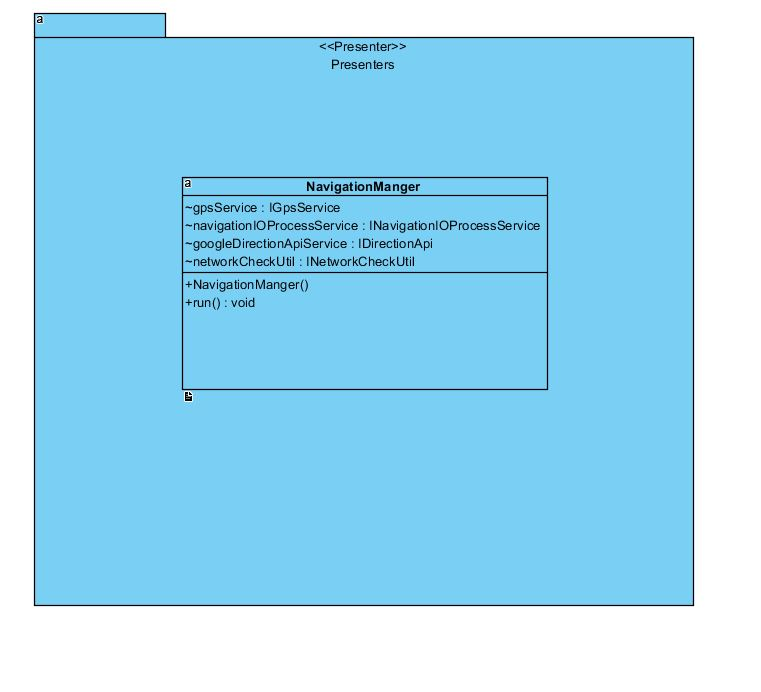
\includegraphics[scale=0.6]{grafiken/liskov.jpg}
        \caption{Class Diagram: Design of the NavigationManager}
        \label{fig:navigationManagerClassDiagram}
    \end{figure}